\documentclass{deliverablereport}
\usepackage{pdfpages}

\usepackage[style=alphabetic,backend=bibtex]{biblatex}
\addbibresource{../../lib/kbibs/kwarcpubs.bib}
\addbibresource{../../lib/kbibs/extpubs.bib}
\addbibresource{../../lib/kbibs/kwarccrossrefs.bib}
\addbibresource{../../lib/kbibs/extcrossrefs.bib}
\addbibresource{../../lib/deliverables.bib}
%\addbibresource{../../lib/publications.bib}
\addbibresource{rest.bib}
% temporary fix due to http://tex.stackexchange.com/questions/311426/bibliography-error-use-of-blxbblverbaddi-doesnt-match-its-definition-ve
\makeatletter\def\blx@maxline{77}\makeatother

\deliverable{component-architecture}{scscp-sage}
\deliverydate{02/27/2017}
\duedate{02/27/2017 (Month 18)}
\def\pn{OpenDreamKit}
\author{ }

\begin{document}
\maketitle
%  Work Package WP6 develops a novel, foundational, knowledge-based framework for
  interfacing existing open source mathematical software systems and knowledge bases into
  a mathematical VRE, where systems can delegate functionalities among each other
  seamlessly without losing semantics.

  The overall Math-in-the-Middle (MitM) Framework developed in WP6 over the last three
  years is described in D6.5; this Report complements it by describing the curated
  contents Math-in-the-Middle (MitM) Ontology which serves as a reference and pivotal
  point for translations between the various input languages of mathematical software
  systems and knowledge bases.

  In a nutshell, the MitM Ontology describes the mathematical objects, concepts, and their
  relations in a general, system-agnostic way in an OMDoc/MMT theory graph while the
  mathematical systems export API theories that describe the system interface language in
  terms of types, classes, constructors, and functions -- again in OMDoc/MMT. These two
  levels of descriptions are linked by OMDoc/MMT alignments that allow the translation of
  expressions between systems.

%%% Local Variables:
%%% mode: visual-line
%%% fill-column: 5000
%%% mode: latex 
%%% TeX-master: "report"
%%% End:

% TODO: replace GitHub issue description by the abstract?
\strut\githubissuedescription
\newpage\tableofcontents\newpage

\section{Introduction}\label{intro}

{\sf SCSCP} stands for the 
{\bf Symbolic Computation Software Composability Protocol}
-- the remote procedure call framework by which different
software components (primarily mathematical software systems) 
may offer computational services to a variety of possible
clients, such as, for example:
\begin{itemize}
\item A computer algebra system (CAS) running on the same computer system or remotely
\item Another instance of the same CAS (in a parallel computing context)
\item A simplistic SCSCP client (e.g. C/C++/Python/etc. program) with a minimal 
SCSCP support needed for a particular application
\item An internet application providing user interface to the computational services
\item A Web server which passes on the same services as Web services to other applications
\item Cloud middleware
\end{itemize}

SCSCP has been developed in the EU FP6 project 026133 
``SCIEnce -- Symbolic Computation Infrastructure for Europe''
(\url{http://www.symbolic-computing.org/}).
In the duration of the project (2006-2011) and subsequent
years, native implementations of SCSCP client and server appeared in
several CAS such as GAP, KANT, Macaulay2, Maple, Mathematica, MuPAD
and TRIP; furthermore, APIs for Java, C and C++ were developed
to facilitate SCSCP implementations in other applications
(see the full list and links at \url{http://www.symbolic-computing.org/}).
However, there were no Python OpenMath SCSCP implementations
(except a prototype quality client supporting only lists of integers)
and that hindered further extension of the SCSCP framework.

In this report we give an overview of work under the task T3.2 
to support SCSCP in all relevant components, necessary to be able
to build interfaces between different systems. 


\section{Systems}\label{systems}

Under the task T3.2, our goal is to make SCSCP-compliant all
relevant components. Since SCSCP is a protocol in which 
both data and instructions are encoded in OpenMath, its
implementation is typically split into two components: 
\begin{itemize}
\item OpenMath support to be able to parse and 
generate OpenMath code and encode/decode mathematical objects
\item client and server functionality needed to establish connection
and exchange with procedure calls and their results.
\end{itemize}

In order to achieve maximal impact on the Python ecosystem, 
instead of implementing SCSCP directly in SageMath, our approach
was to provide independent Python libraries, which may be used not
only in SageMath but also in a number of other Python applications
including scientific computing libraries such as e.g. 
SciPy, NumPy, SymPy etc.



\subsection{Python, SageMath and its components}

OpenMath and SCSCP support in Python is provided by two libraries, 
{\sf openmath} and {\sf scscp}, which are available from PyPI at
\url{https://pypi.python.org/pypi/openmath/} and
\url{https://pypi.python.org/pypi/scscp/} and
may be installed using the standard {\sf pip} installer 
both under Python 2 and Python 3. The development repositories
and issue trackers for these packages are hosted on GitHub
at \url{https://github.com/OpenMath/py-openmath}
and \url{https://github.com/OpenMath/py-scscp}.

TODO: Ask Luca for more detailed overview of the design of 
\url{https://github.com/OpenMath/py-scscp} 
and \url{https://github.com/OpenMath/py-openmath}. 

Explain how the user can now use these packages to extend supported OpenMath CDs
or use private encodings and implement own remote procedures.

TODO: Appendix with READMEs from \url{https://github.com/OpenMath/py-scscp}
and \url{https://github.com/OpenMath/py-openmath}. The latter should have
some more detailed README.

What other systems are doing? Because SageMath interfaces them, to offer them
as remote services, the SCSCP server can be run in SageMath, and Sage may be
also an SCSCP client, so can steer computation talking to e.g. remote GAP 
via SCSCP and local PARI/GP or Singular via its own interface.

We provide more details and examples of usage for the SCSCP client and server in
Python in Appendices. 

Appendix \ref{python2-to-GAP} shows an example of Python 2 client connecting
to a GAP server.

Appendix \ref{python3-to-GAP} shows an example of Python 3 client connecting
to a GAP server.

Appendix \ref{SageMath-to-GAP} shows an example of Python 3 client connecting
to a GAP server.



\subsection{GAP}

TODO: add URLs

OpenMath and SCSCP support in GAP is provided by two GAP packages, 
{\sf OpenMath} and {\sf SCSCP}. This packages are included in the 
standard GAP distribution and are also available from their 
websites \url{https://gap-packages.github.io/openmath/} and
\url{https://gap-packages.github.io/scscp/}. 
The development repositories and issue trackers for these packages are hosted on GitHub
at \url{https://github.com/gap-packages/scscpopenmath}
and \url{https://github.com/gap-packages/scscp}.

The OpenMath package provides encoding/decoding, and supports both XML and binary OpenMath.
The SCSCP package implements SCSCP client and server, and on top of
that provides a framework for distributed parallel computations.

TODO: more details and either URLs of manuals or append them to the report?

During the reported period, we have prepared new versions of 
both packages and migrated their development repositories and
websites under the GAP packages VO on GitHub. 
Their new versions are now picked up for the redistribution
with GAP and will appear in the next GAP release. Major changes
were upgrades and compatibility fixes for next GAP releases, 
and improvements to improve the security and robustness when
running public SCSCP servers. 

TODO: release GAP 4.8.7 by the end of February?

Several examples of using GAP SCSCP client and server are given
in the next section. They show how GAP SCSCP support feeds into
activities from other workpackages (Docker, databases).


\subsection{MMT/MathHub}

TODO: Ask Tom to provide a description


\section{Examples}\label{examples}

TODO: introduction to this section. Alternatively, just incorporate 
examples into appropriate Systems (sub)sections.

\subsection{GAP SCSCP server in Docker container}

A very efficient and secure way to run public GAP SCSCP
server is to run it in the GAP docker container. Under the
Task ??? we have established a pipeline of GAP Docker 
containers, and the README for the container for GAP and
packages \url{https://hub.docker.com/r/gapsystem/gap-docker/}
is shown in Appendix \ref{SCSCP-with-GAP-docker} and explains
how to start GAP SCSCP server in the container.
TODO:more instructions here. Why useful - because some packages
are difficult to install otherwise.


\subsection{Number of groups of order $n$}\label{gnu-reproducibility}

TODO: describe \url{https://github.com/alex-konovalov/gnu} which provides
an SCSCP server for the number of isomorphism types of groups. Provide
a GAP Jupyter notebook that talks to that server in the appendix.


\subsection{SageMath}

TODO: brief description, and reference to the appendix, extend examples


\subsection{Singular}

TODO: Sebastian?


\subsection{PARI/GP}

TODO: Via SageMath?
% http://doc.sagemath.org/html/en/reference/interfaces/sage/interfaces/gp.html


\subsection{Parallel SCSCP tutorial}

TODO: describe \url{https://github.com/alex-konovalov/scscp-demo},
include page in the appendix. Was taught twice at CoDiMa training schools.

\section{Future work}

Dissemination: reach out to SciPy, SymPy, NumPy communities.

Under the ODK project, we transferred SCSCP specification
to OpenMath society and licensed it under
W3C Software and document notice and license.

Make a proper webpage for SCSCP under OpenMath VO, with
PDFs of the specification and links to existing implementations.
TODO: give URLs of the new SCSCP website and repository.



\printbibliography

\appendix

\section{Example: SCSCP client in Python2 connecting to GAP server}\label{python2-to-GAP}
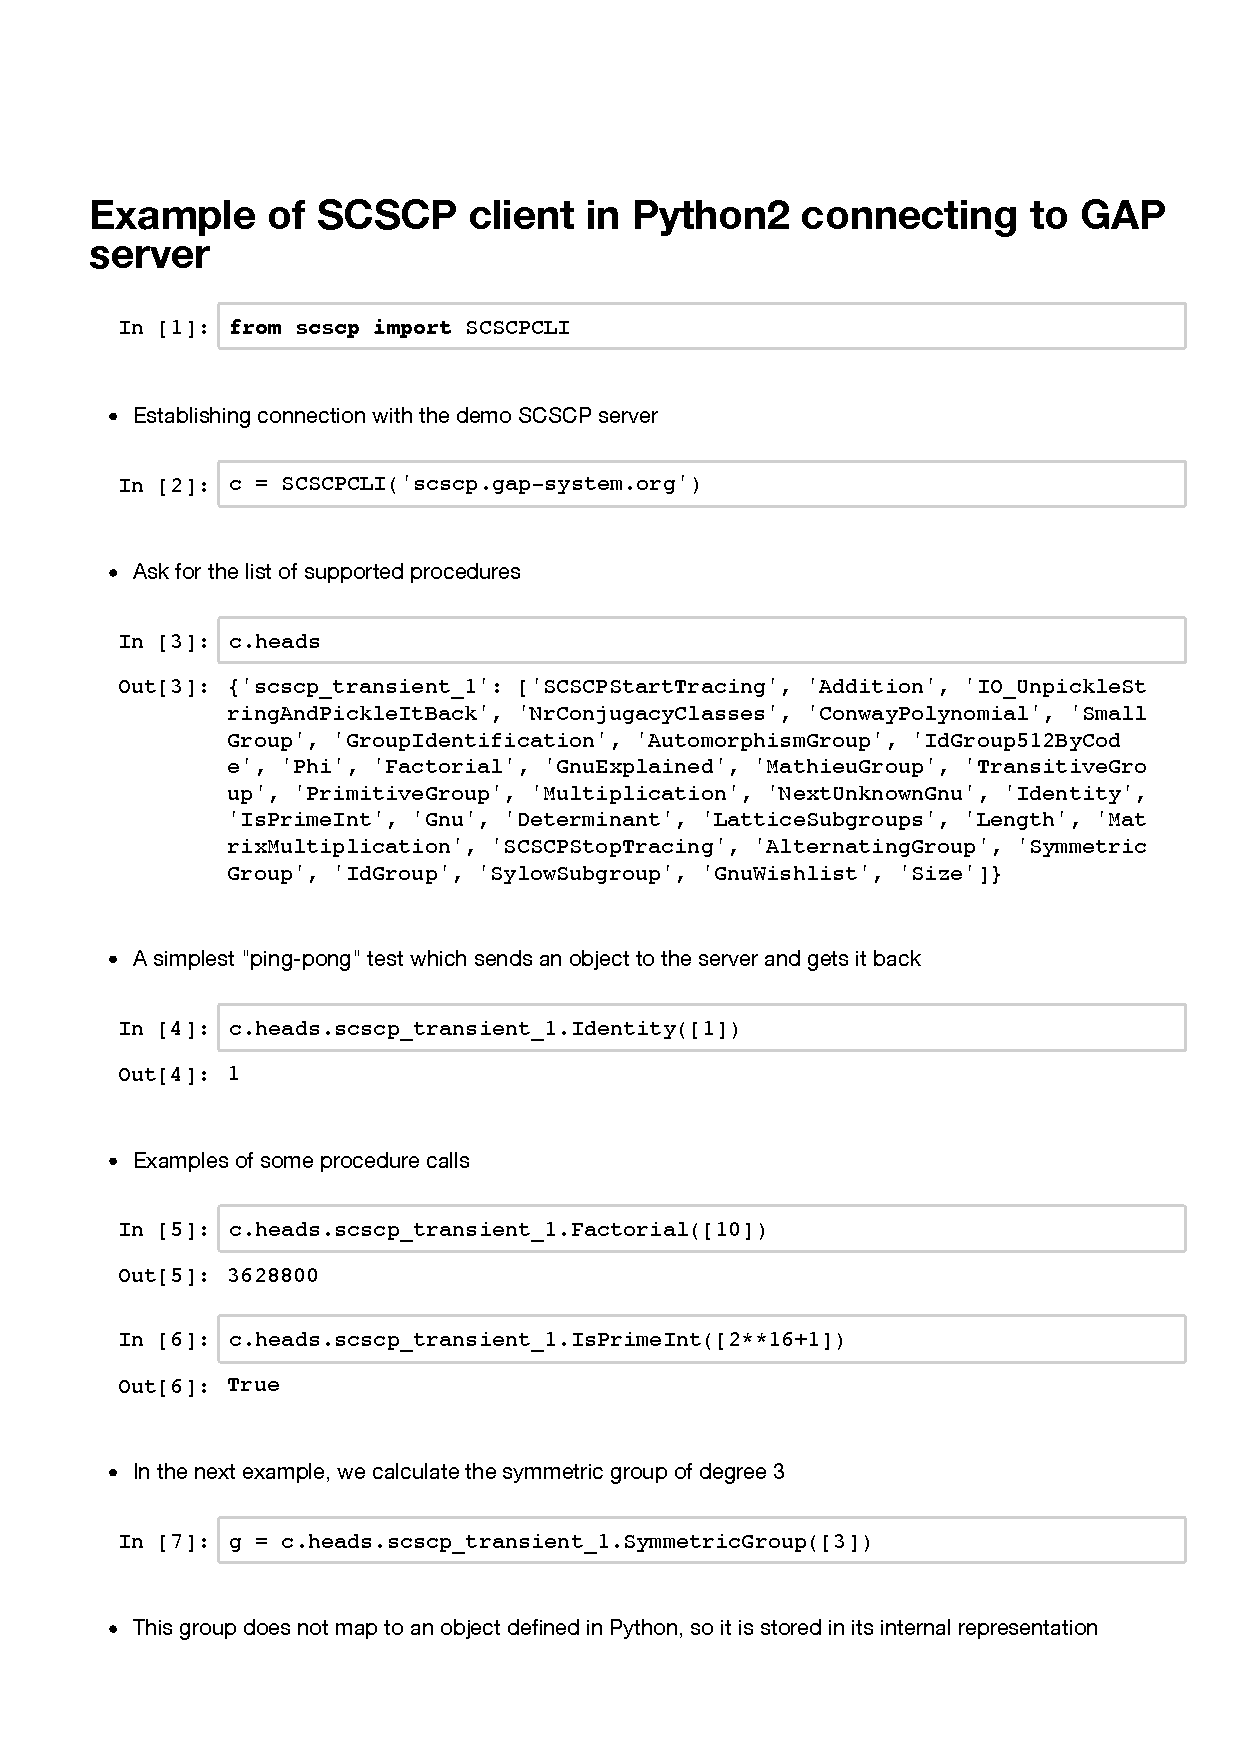
\includepdf[pages=-,scale=0.9,pagecommand={}]{examples/Python2-to-GAP.pdf}

\section{Example: SCSCP client in Python3 connecting to GAP server}\label{python3-to-GAP}
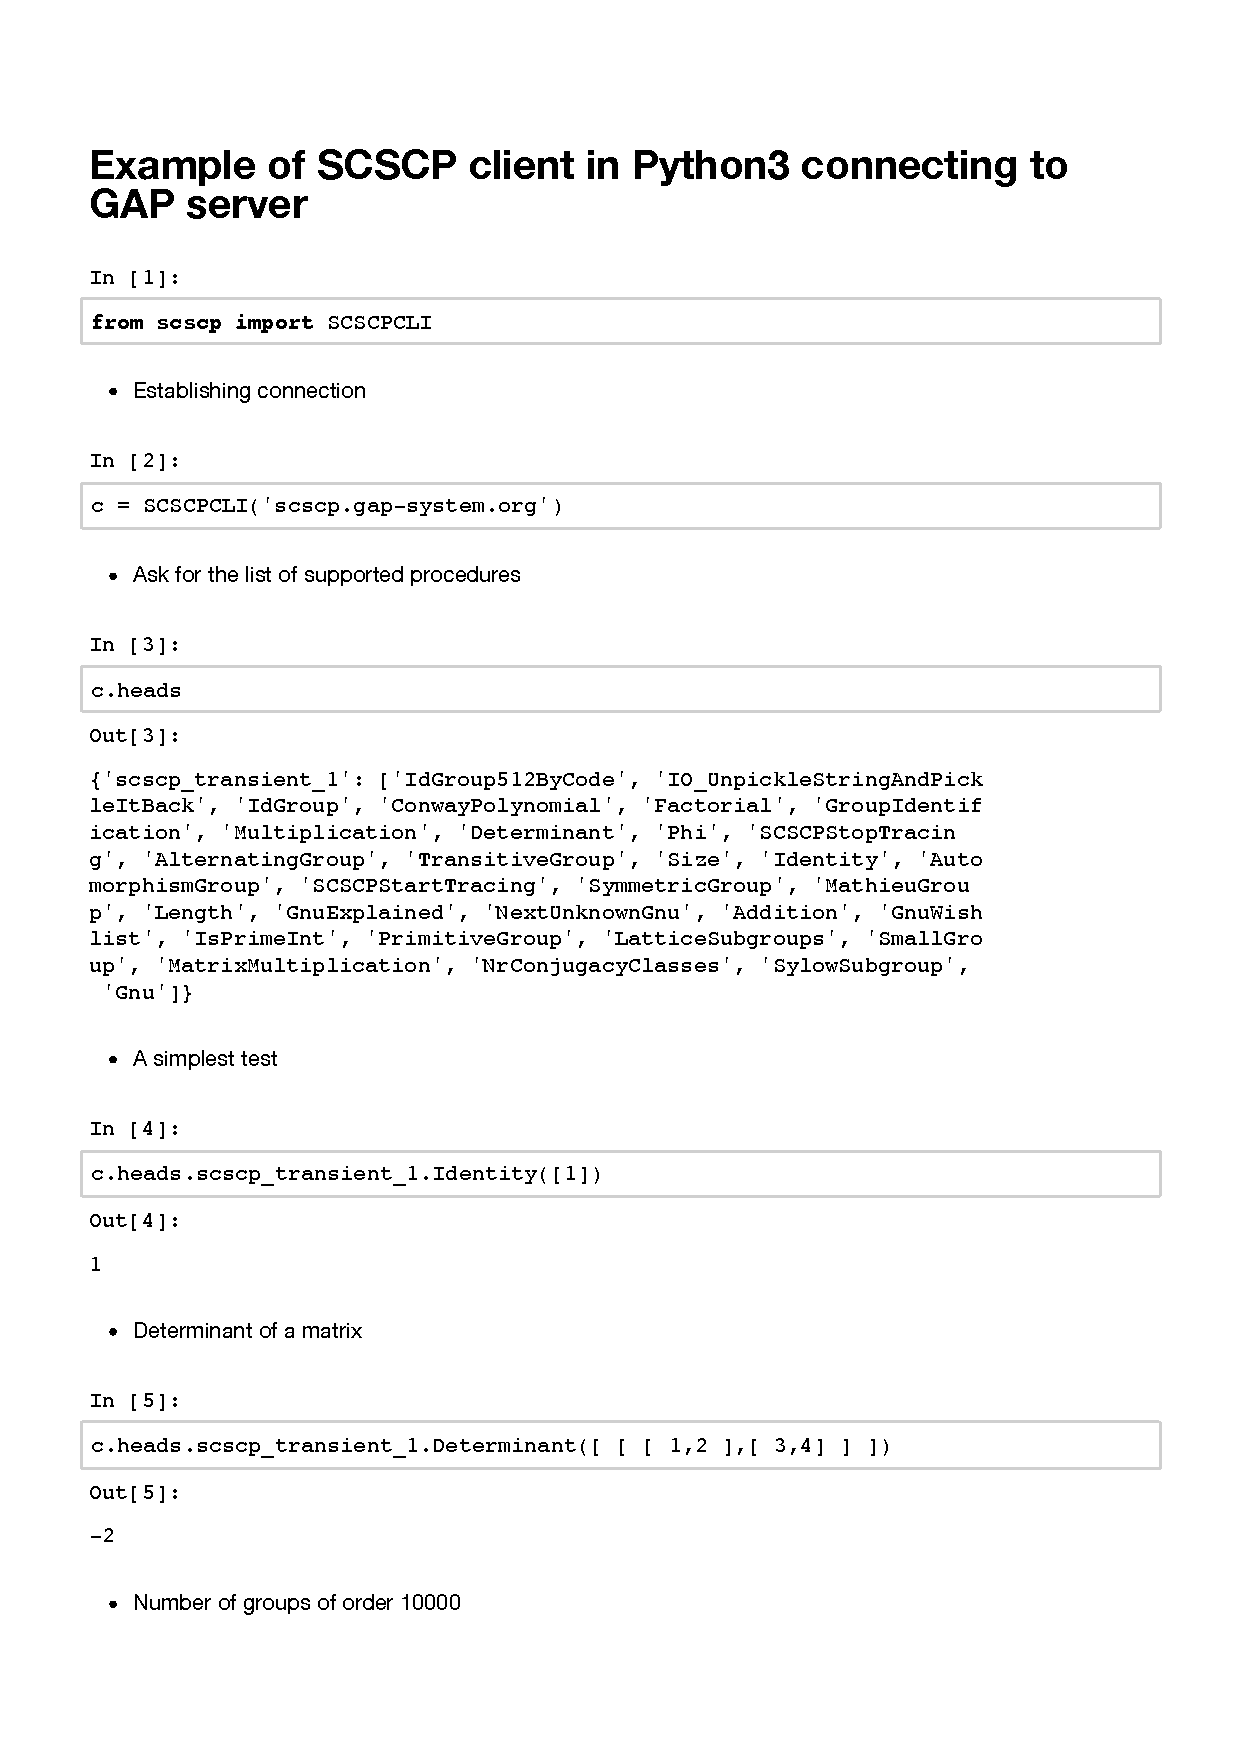
\includepdf[pages=-,scale=0.9,pagecommand={}]{examples/Python3-to-GAP.pdf}

\section{Example: SCSCP client in SageMath connecting to GAP server}\label{SageMath-to-GAP}
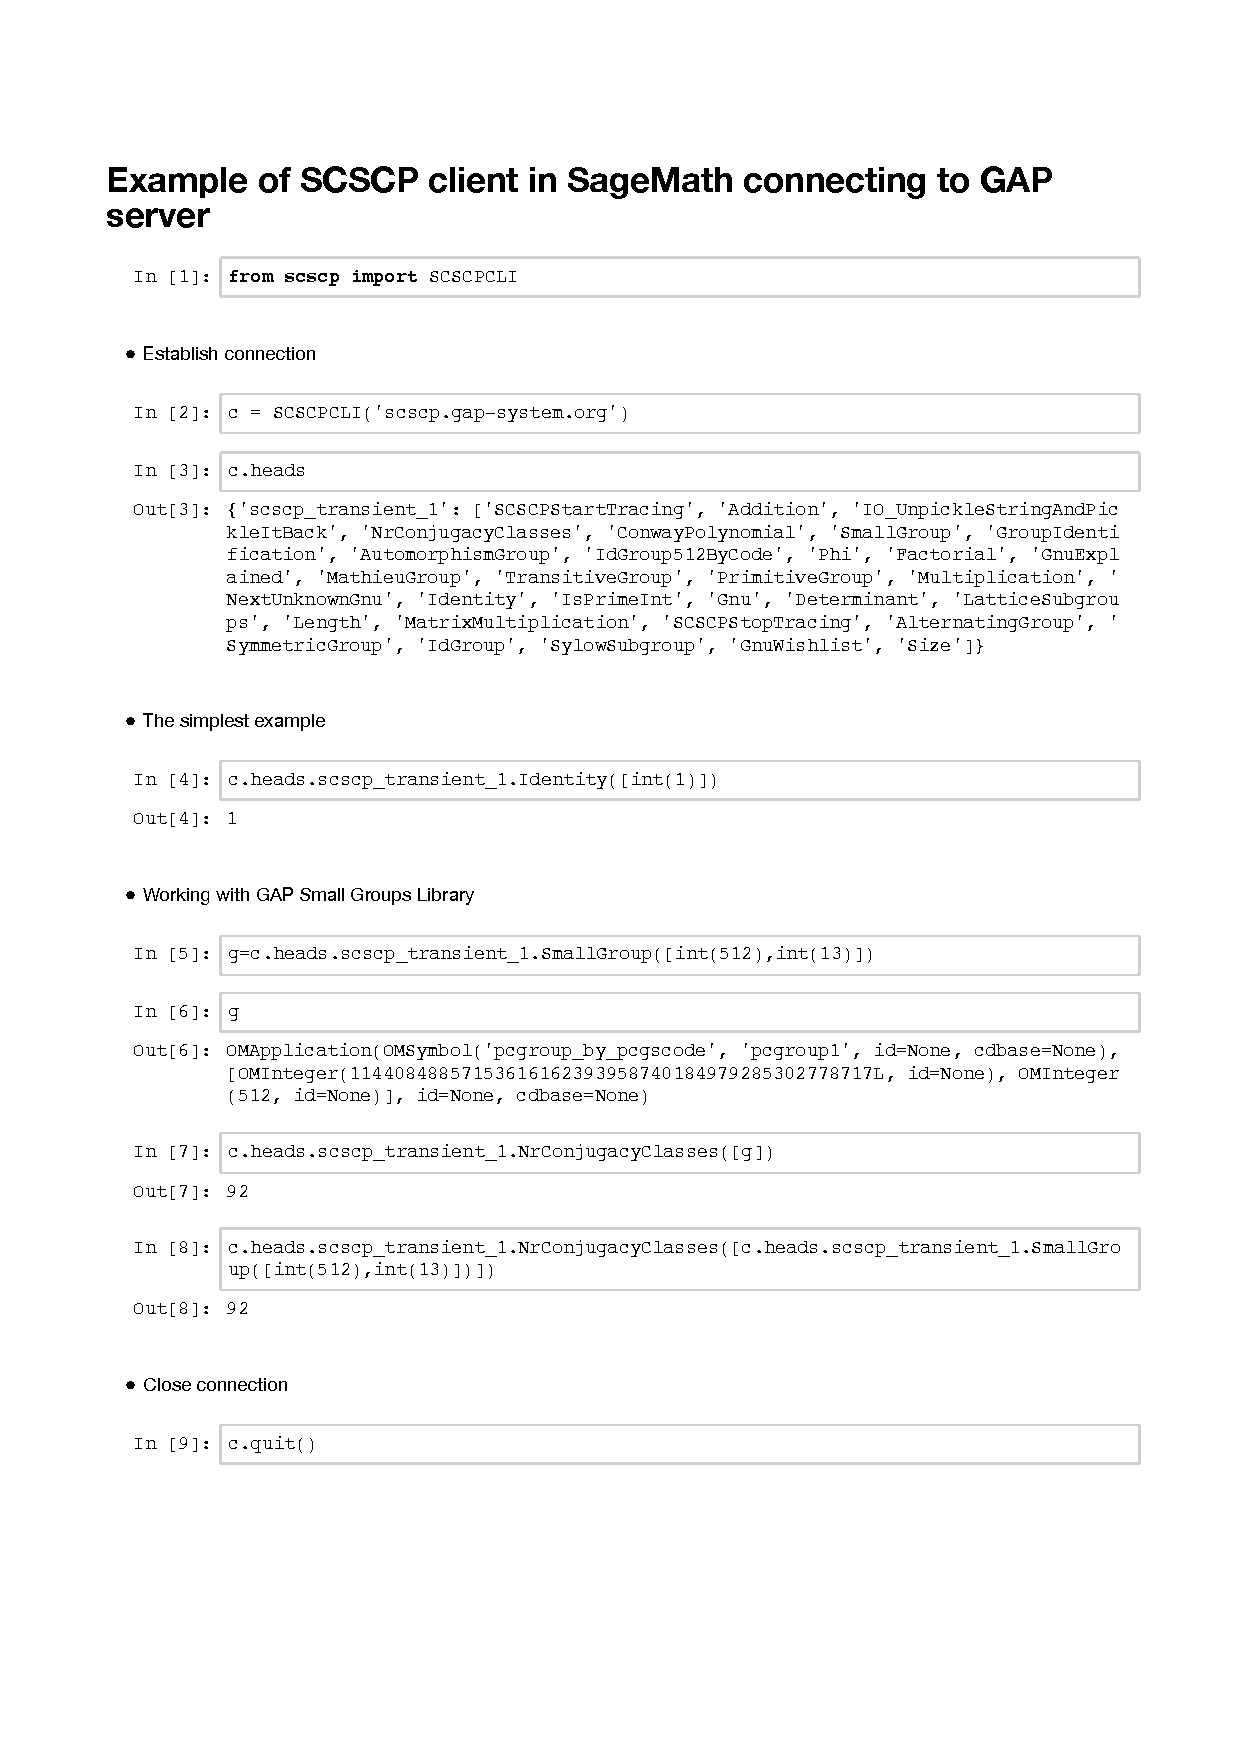
\includepdf[pages=-,scale=0.9,pagecommand={}]{examples/SageMath-to-GAP.pdf}

\section{Documentation for the GAP Docker container}\label{SCSCP-with-GAP-docker}
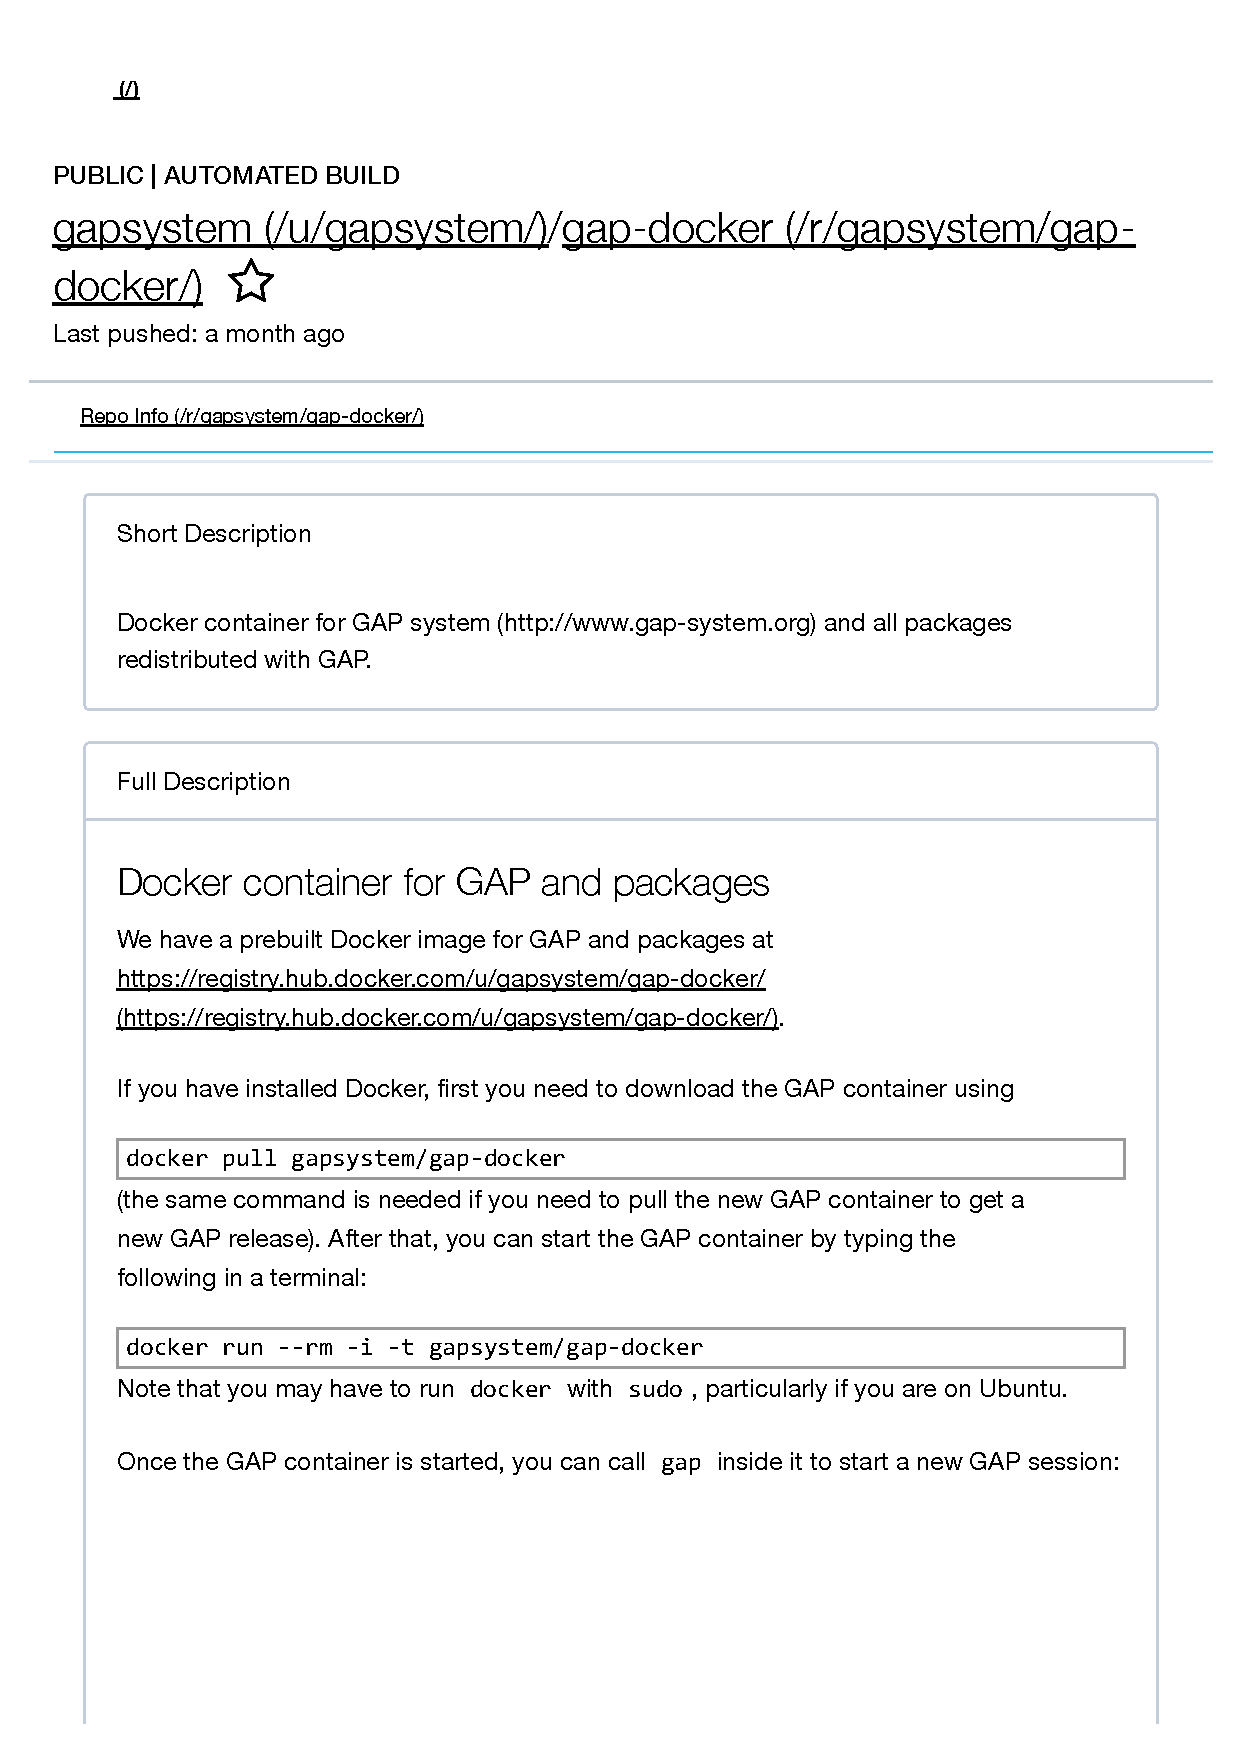
\includepdf[pages=-,scale=0.8,pagecommand={}]{examples/SCSCP-with-GAP-docker.pdf}

\section{Documentation for the GAP SCSCP server for the number of isomorphism types of groups of order $n$}\label{Gnu-SCSCP-server}
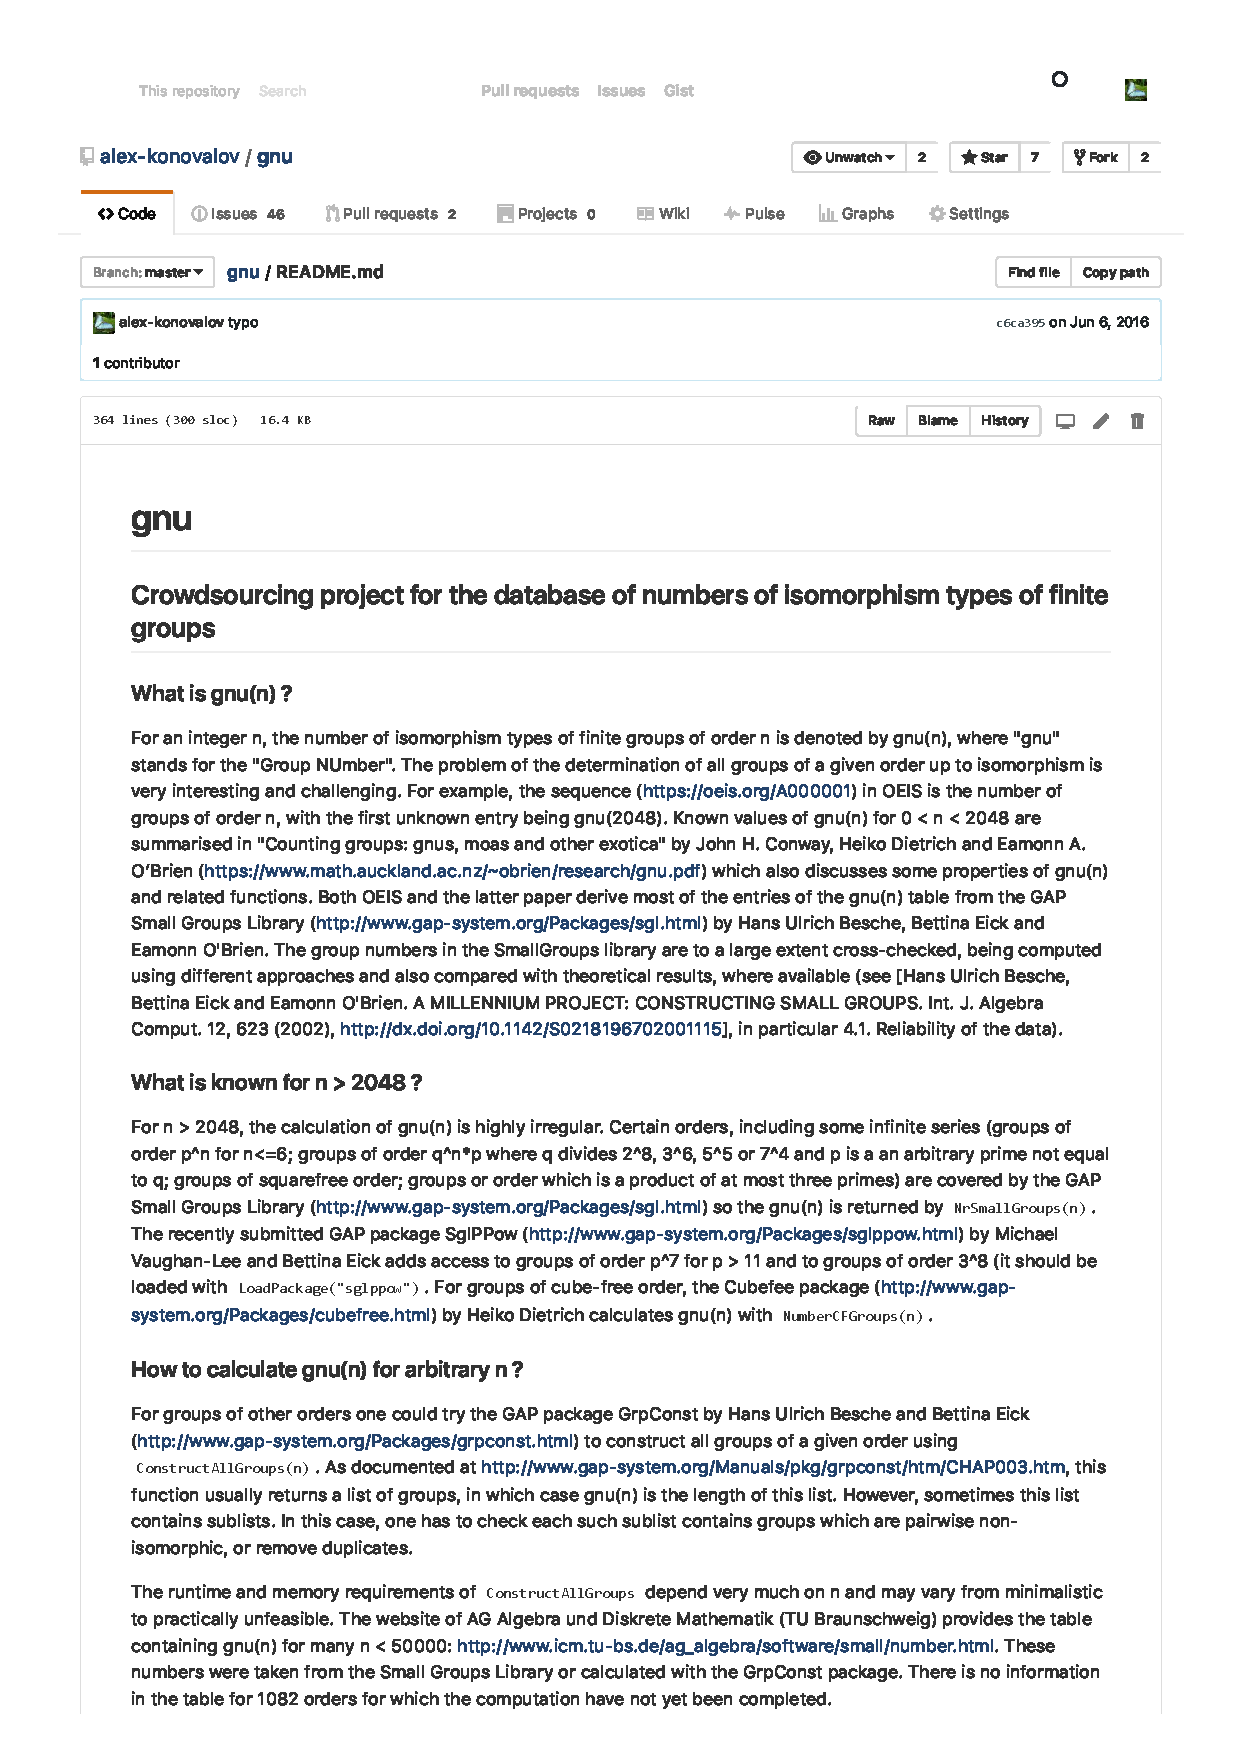
\includepdf[pages=-,scale=0.9,pagecommand={}]{examples/Gnu-SCSCP-server.pdf}

%TODO: Do we need to include manuals of GAP OpenMath and SCSCP packages?
%(20 and 54 pages respectively?)
%\section{Documentation for GAP package OpenMath}
%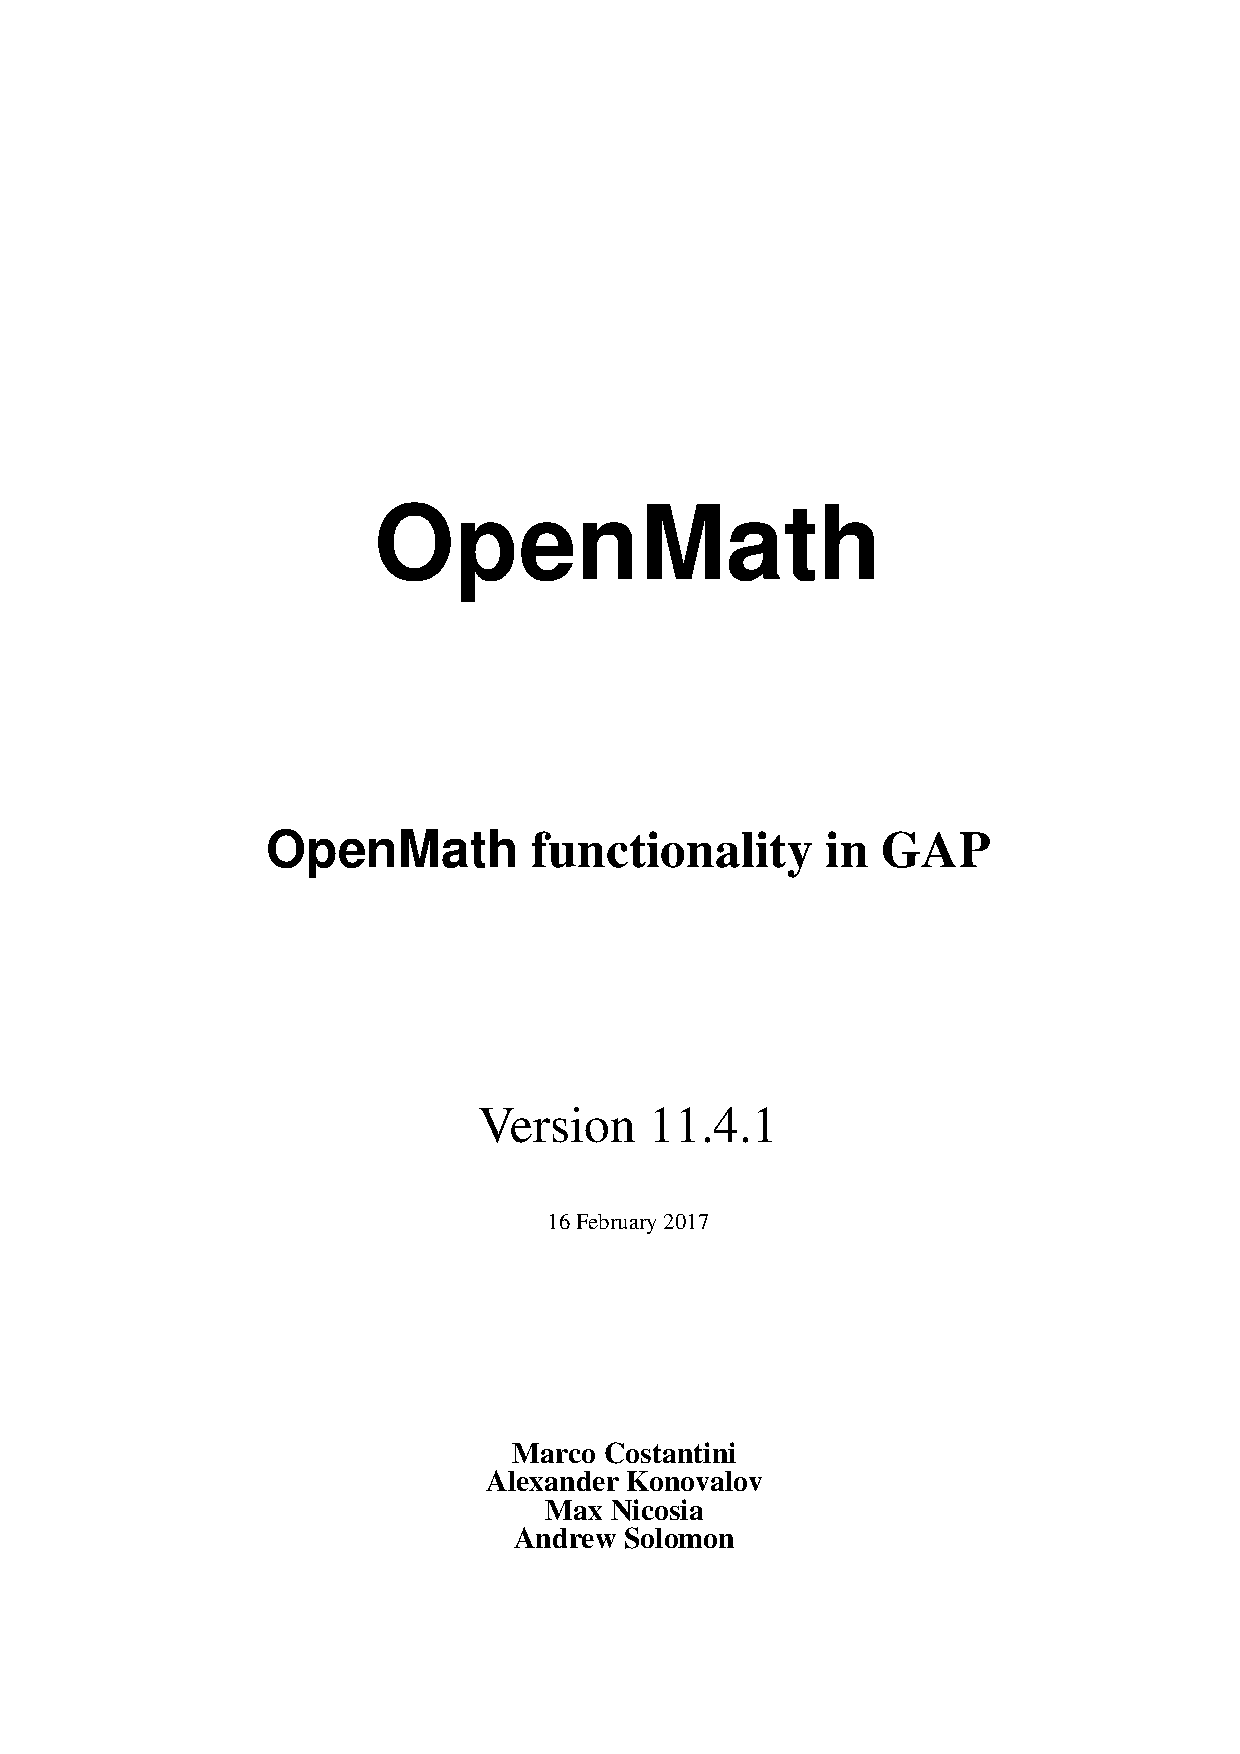
\includepdf[pages=-]{manuals/gap-openmath.pdf}
%\section{Documentation for GAP package SCSCP}
%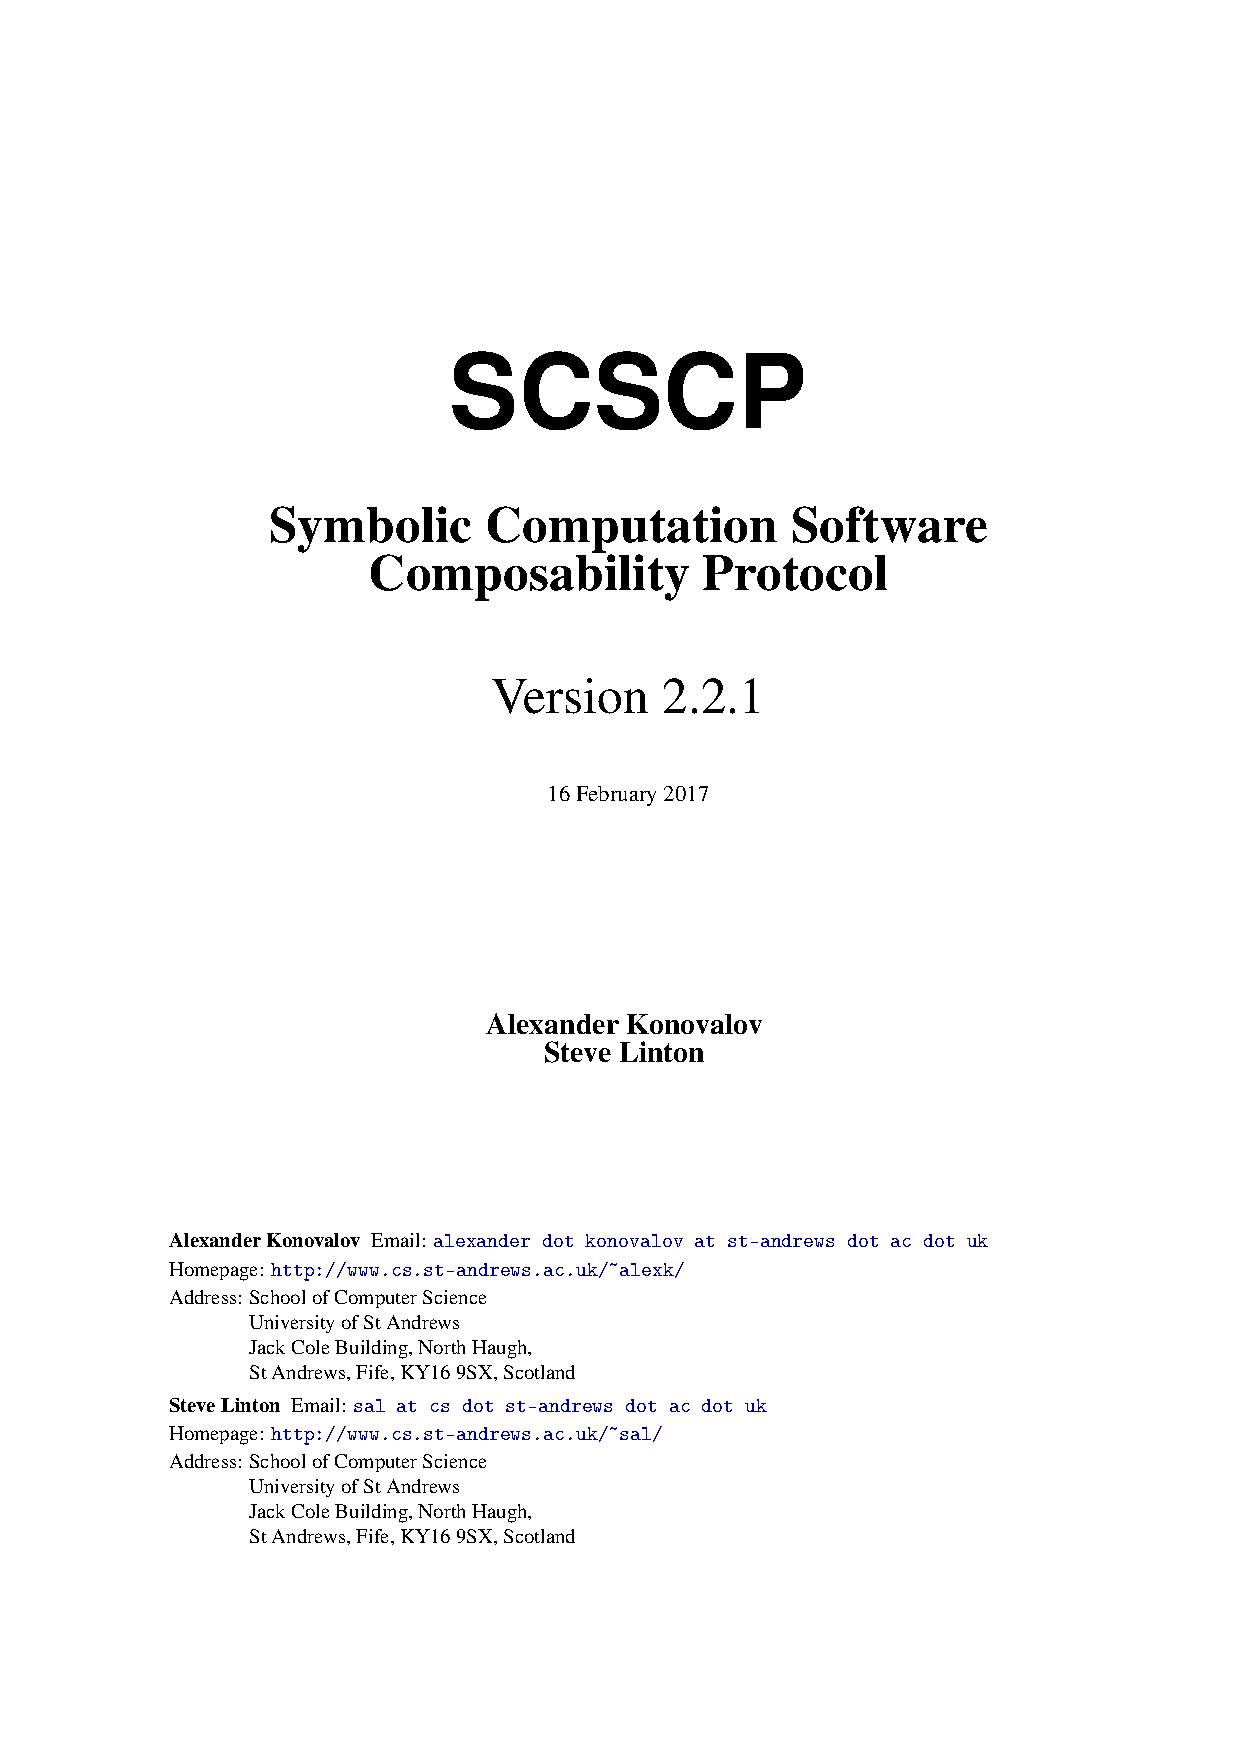
\includepdf[pages=-]{manuals/gap-scscp.pdf}

\end{document}

%%% Local Variables:
%%% mode: latex
%%% TeX-master: t
%%% End:

%  LocalWords:  githubissuedescription newpage tableofcontents newpage printbibliography
